\documentclass[11pt]{article}

% ── Packages ────────────────────────────────────────────────
\usepackage[margin=1in]{geometry}
\usepackage{amsmath, amssymb, amsthm}
\usepackage{booktabs}
\usepackage{graphicx}
\usepackage{hyperref}
\usepackage{natbib}
\usepackage{setspace}
\usepackage{microtype}
\usepackage{enumitem}
\usepackage{caption}
\usepackage{subcaption}
\usepackage{xcolor}
\usepackage{float}
% code packages
\usepackage{listings}
\usepackage{inconsolata}
\lstset{basicstyle=\ttfamily\footnotesize,breaklines=true}
\usepackage{csvsimple}
\usepackage{booktabs}

% ── Hyperref setup ──────────────────────────────────────────
\hypersetup{
    colorlinks = true,
    linkcolor  = black,
    citecolor  = black,
    urlcolor   = blue
}

% ── Theorem environments ────────────────────────────────────
\newtheorem{theorem}{Theorem}
\newtheorem{proposition}{Proposition}
\newtheorem{lemma}{Lemma}
\newtheorem{corollary}{Corollary}
\theoremstyle{definition}
\newtheorem{definition}{Definition}
\newtheorem{assumption}{Assumption}
\theoremstyle{remark}
\newtheorem{remark}{Remark}

% ── Spacing ─────────────────────────────────────────────────
\onehalfspacing

% ── Title block ─────────────────────────────────────────────
\title{Love of Variety Simulation}
\author{Tate Mason}
\date{\today}

% ============================================================
\begin{document}
\maketitle
\thispagestyle{empty}

% ── Abstract ────────────────────────────────────────────────

\newpage
\setcounter{page}{1}

\section{Model}
The consumer's problem is to maximize utility subject to their choice set. The utility function is as follows:

\begin{equation}
  U_{ijt} = \beta_i \cdot X_{jt} - \gamma_{ijt}(X_{jt} - \bar{X}_{jt})^2 + \epsilon_{ijt}
\end{equation}

Where $U_{ijt}$ is the utility of consumer $i$ for product $j$ at time $t$, $\beta_i$ is the consumer's sensitivity to the product's attributes, $X_{jt}$ is the attribute of product $j$ at time $t$, $\gamma_ijt$ is the consumer's sensitivity to sameness of the product's attribute from its average, $\bar{X}_{jt}$ is the average attribute of product $j$ at time $t$, and $\epsilon_{ijt}$ is a random error term distributed T1EV.

The consumer chooses the product that maximizes their utility. The choice set includes all products available in the market at time $t$. The probability of consumer $i$ choosing product $j$ at time $t$ can be expressed as:
\begin{equation}
  P_{ijt} = \frac{e^{U_{ijt}}}{\sum_{k} e^{U_{ikt}}}
\end{equation}

Where the denominator sums over all products $k$ in the choice set at time $t$.

The simulation will involve setting $\beta$ and $\gamma$ at differing levels to observe how consumer choices change.

Further, we will look at the basics of the firm's decision of what to present to the consumer. The firm will "send" three products each period. Define $C_t = \{c_1, c_2, c_3\}$ as the set of products the firm sends at time $t$.
$C_t \sim N(\bar{X_{j,t}}, \simga_x)$ where $\bar{X_{j,t}}$ is the average attribute of product $j$ at time $t$ and $\sigma_x$ is the standard deviation of the attributes of the products sent by the firm. We want to 
see how the firm will react to various regimes in terms of $\sigma_x$ and how that will affect consumer choices.

\section{Results}

\subsection{Consumer Choices and Utility}
\begin{centering}
  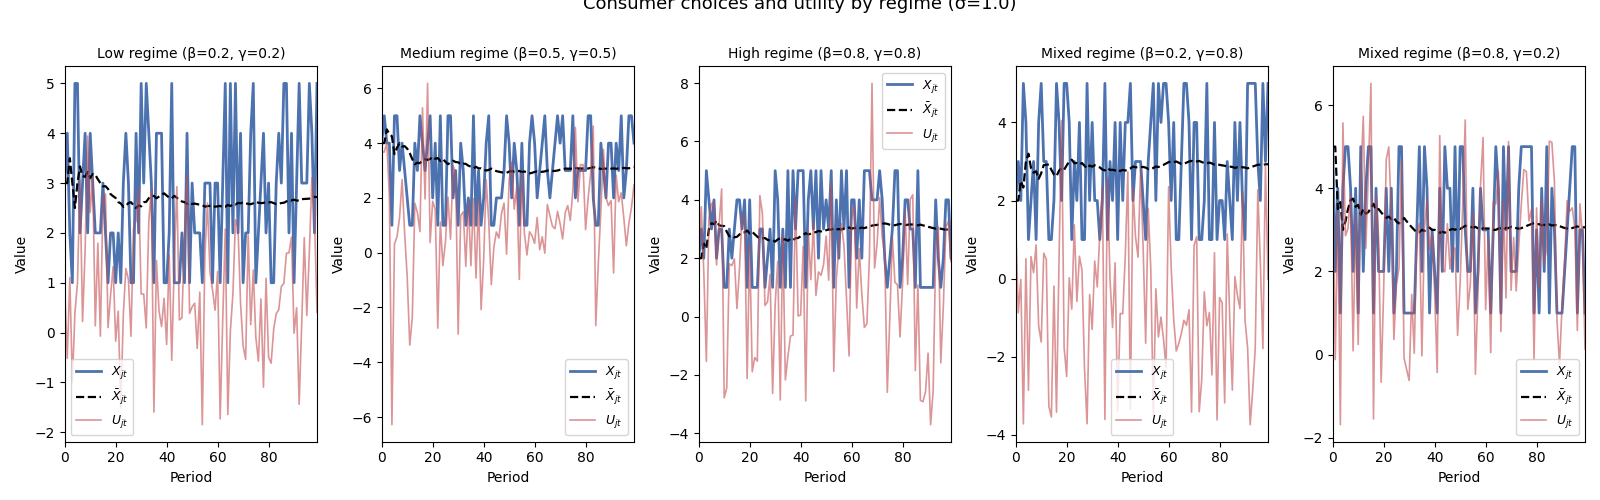
\includegraphics[width=\textwidth]{../../Output/consumer_choices_and_utility_by_regime.png}
\end{centering}

The blue line represents the chosen product attribute at time $t$. The orange line represents the utility from that period. The black dashed line is the evolution of the mean attribute. From the figures, we can see that in the
low regime, it seems that after about 50 periods, we converge to a "steady state" where utiility is in line with the chosen attribute, implying in this case they have been able to find the "sweet spot". In the medium regime,
It takes closer to 75 periods, with a lot of volatility even until the 70th or so period. In this period the "sweet spot" is less clear, as there is still lower utility than attribute value. In the high regime, we actually see a 
decent fit, but with spikes intermittently. This is likely because when the consumer is more sensitive to variety, the deviations will be more pronounced. They also like what they like more, so this creates an interesting dynamic
where they want newness (which they may like), but if it is too new they'll be punished. In the regime with low utility from characteristic and a higher variety parameter, we cannot get a good fit, with utility going all over the place,
especially in a negative direction. This is likely because the consumer is very sensitive to newness, and any new draw of $\sigma_x$ that is too high will cause a sharp drop in utility. In the inverse regime, we see almost the exact opposite,
though with an admittedly better fit to the $X_{jt}$ chosen. Here, this is likely because the consumer is just happy to have new product characteristics, and is relatively insensitive to redundancy in product characteristics. This is why
we see positive spikes in utility. 

All in all, we see that utility is more volatile as $X_{jt}$ deviates from $\bar{X}_{jt}$, a data fact we should expect. We also see that the initial parameters of the consumer have a large effect of the model.

\subsection{Rolling Variance of Consumer Choices and $\sigma_x$}
\begin{centering}
  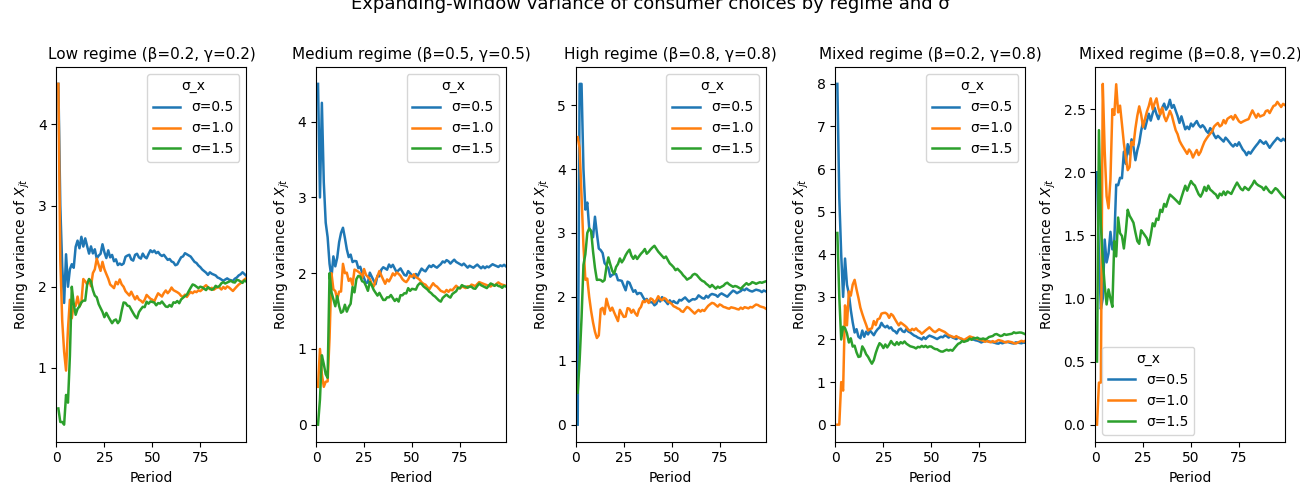
\includegraphics[width=\textwidth]{../../Output/rolling_variance_of_consumer_choices_by_regime_and_sigma.png}
\end{centering}

Now, we can discuss the rolling variance of $\sigma_x$. I set it to 3 starting values $\sigma_x = [0.5, 1.0, 1.5]$. Starting in the low regime, the high value of $\sigma_x$ grows in variance over the entire time horizon while the middle and low 
value reach steady state after about 40-50 periods. In the medium regime, they converge similarly, with $\sigma_x = 1.5$ having decreasing variance for the first 10 or so periods. The middle and low values do not really evolve, staying fairly
constant over the time horizon. In the high regime, All three values grow in variance, but the high value grows the entire time while the other two converge after about 25-35 periods. In the regime with $\beta=0.2, \gamma=0.8$, the high value of
the high value grows the entire time, while the other two almost immediately converge to a steady state. In the inverse regime, the high variance falls immediately, before climbing back for about 10 periods, then falling for 20 periods and then 
converging. The other two converge after about 10 periods.

Here, it seems that without high variance, sigma is not super volatile regardless of regime. When variance is high, however, it is very volatile with respect to $\gamma$ especially. This is likely because when the consumer is more sensitive 
to variety, deviations will be more pronounced and so the variance of $\sigma_x$ will be more volatile. 

\section{Code}
\lstinputlisting[language=Python]{../../Code/init_sim.py}

\end{document}
